% Created 2019-10-07 Mon 19:16
% Intended LaTeX compiler: pdflatex
\documentclass[11pt, compress, aspectratio=169, xcolor={table,usenames,dvipsnames}]{beamer}

\usepackage{booktabs}
\renewcommand\maketitle{}
\usepackage{roboto}
\usepackage{booktabs}
\usepackage{ragged2e}
\usepackage{array}
\usepackage{listings}
\usepackage{times}
\usepackage{graphicx}
\usepackage[english]{babel}
\usepackage{multicol}
\usepackage[scale=2]{ccicons}
\usepackage{url}
\usepackage{relsize}
\usepackage{amsmath}
\usepackage{bm}
\usepackage{wasysym}
\usepackage{ragged2e}
\usepackage{textcomp}
\usepackage{pgfplots}
\usepgfplotslibrary{dateplot}
\definecolor{Base}{HTML}{191F26}
\definecolor{Accent}{HTML}{157FFF}
\setbeamercolor{alerted text}{fg=Accent}
\setbeamercolor{frametitle}{bg=Base}
\setbeamercolor{normal text}{bg=black!2,fg=Base}
\setsansfont[BoldFont={Roboto},Numbers={OldStyle}]{Roboto}
\lstdefinelanguage{Julia}%
  {morekeywords={abstract,struct,break,case,catch,const,continue,do,else,elseif,%
      end,export,false,for,function,immutable,mutable,using,import,importall,if,in,%
      macro,module,quote,return,switch,true,try,catch,type,typealias,%
      while,<:,+,-,::,/},%
   sensitive=true,%
   alsoother={$},%
   morecomment=[l]\#,%
   morecomment=[n]{\#=}{=\#},%
   morestring=[s]{"}{"},%
   morestring=[m]{'}{'},%
}[keywords,comments,strings]%
\lstset{ %
  backgroundcolor={},
  basicstyle=\ttfamily\scriptsize,
  breakatwhitespace=true,
  breaklines=true,
  captionpos=n,
  commentstyle=\color{Accent},
  extendedchars=true,
  frame=n,
  keywordstyle=\color{Accent},
  language=R,
  rulecolor=\color{black},
  showspaces=false,
  showstringspaces=false,
  showtabs=false,
  stepnumber=2,
  stringstyle=\color{gray},
  tabsize=2,
}
\renewcommand*{\UrlFont}{\ttfamily\smaller\relax}
\graphicspath{{../../img/}}
\addtobeamertemplate{block begin}{}{\justifying}

\usepackage[orientation=portrait,size=a0,scale=1.6]{beamerposter}
\usetheme{LIG-poster}
\usecolortheme{LIG}

\pgfdeclareimage[height=\paperheight,width=\paperwidth]{overlay_image}{../../../img/polaris_color.pdf}
\usebackgroundtemplate{\tikz\node[inner sep=0] {\pgfuseimage{overlay_image}};}
\usetheme{default}
\author{Pedro Bruel - phrb@ime.usp.br}
\date{\today}
\title{Autotuning under Tight Budget Constraints:  \\[0.3em] A Transparent Design of Experiments Approach}
\hypersetup{
 pdfauthor={Pedro Bruel - phrb@ime.usp.br},
 pdftitle={Autotuning under Tight Budget Constraints:  \\[0.3em] A Transparent Design of Experiments Approach},
 pdfkeywords={},
 pdfsubject={},
 pdfcreator={Emacs 26.3 (Org mode 9.2.5)},
 pdflang={English}}
\begin{document}

\maketitle

\begin{frame}
\begin{columns}
\begin{column}{0.89\columnwidth}
\vspace{-0.2em}
\begin{center}
  {\normalsize
    \textit{\alert{Pedro Bruel}$^{1,3}$, Steven Quinito Masnada$^{2}$, Brice
    Videau$^{3}$, Arnaud Legrand$^{3}$, Jean-Marc Vincent$^{3}$, Alfredo Goldman$^{1}$}
  }
\end{center}
\vspace{-0.8em}
\begin{columns}
\begin{column}[t]{0.48\columnwidth}
\begin{block}{Autotuning: Optimizing Program Configurations}
\begin{center}
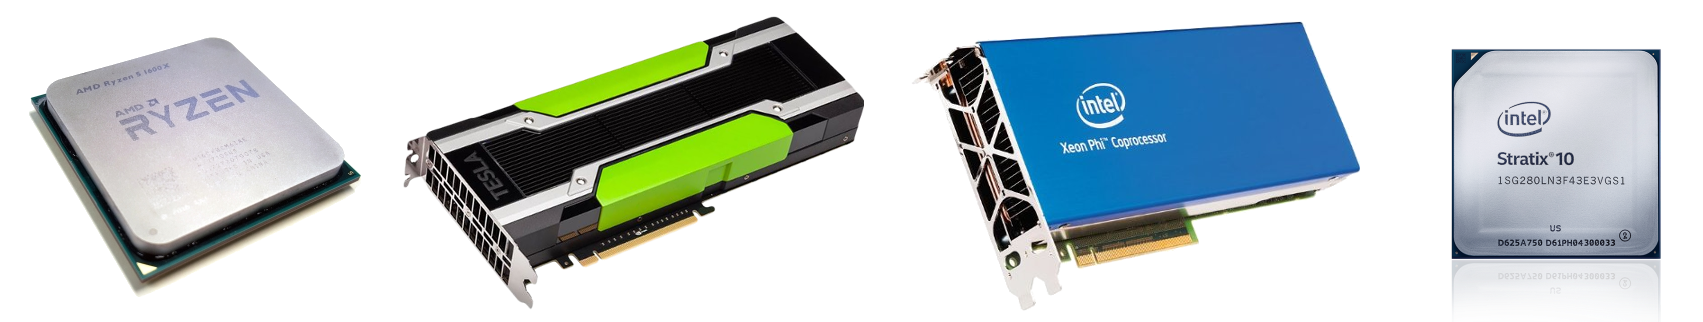
\includegraphics[width=.9\columnwidth]{../../../img/architectures.png}
\end{center}

\begin{itemize}
\item How to write \alert{efficient code} for each of these?
\item We can use \alert{autotuning}: the process of \alert{automatically
finding} a \alert{configuration} of a program that optimizes an
\alert{objective}
\end{itemize}
\end{block}

\begin{block}{Strategies for Exploring Search Spaces}
\begin{columns}
\begin{column}{0.59\columnwidth}
\vspace{0.45em}
{\tiny
\begin{table}
    \centering
    \scriptsize
    \begin{tabular}{@{}lll@{}}
        \toprule
        System & Domain & Approach \\ \midrule
        \rowcolor{red!25} ATLAS & Dense Linear Algebra & Exhaustive\\ \addlinespace
        \rowcolor{green!25} INSIEME & Compiler & Genetic Algorithm \\
        \rowcolor{green!25} Active Harmony & Runtime & Nelder-Mead \\
        \rowcolor{green!25} ParamILS & Domain-Agnostic & Stochastic Local Search \\
        \rowcolor{green!25} OPAL & Domain-Agnostic & Direct Search \\
        \rowcolor{green!25} OpenTuner & Domain-Agnostic & Ensemble \\ \addlinespace
        \rowcolor{cyan!25} MILEPOST GCC & Compiler & Machine Learning \\
        \rowcolor{cyan!25} Apollo & GPU kernels & Decision Trees \\ \addlinespace
        \bottomrule
    \end{tabular}
\end{table}

}
\begin{center}
{\tiny
\colorbox{red!25}{Exhaustive},
\colorbox{green!25}{Meta-Heuristics},
\colorbox{cyan!25}{Machine Learning}
}
\vspace{.5em}
\end{center}
\end{column}

\begin{column}{0.39\columnwidth}
Assumptions:
\vspace{0.3em}
\begin{itemize}
\item \alert{Many measurements}, \alert{``smoothness''}, \alert{reachable solutions}
\vspace{0.3em}
After optimizing:
\vspace{0.3em}
\begin{itemize}
\item \alert{Learn ``nothing''}, \alert{can't explain choices}
\end{itemize}
\end{itemize}
\end{column}
\end{columns}
\end{block}
\end{column}
\begin{column}[t]{0.48\columnwidth}
\begin{block}{Autotuning: Search Spaces are Hard to Explore}
\begin{center}
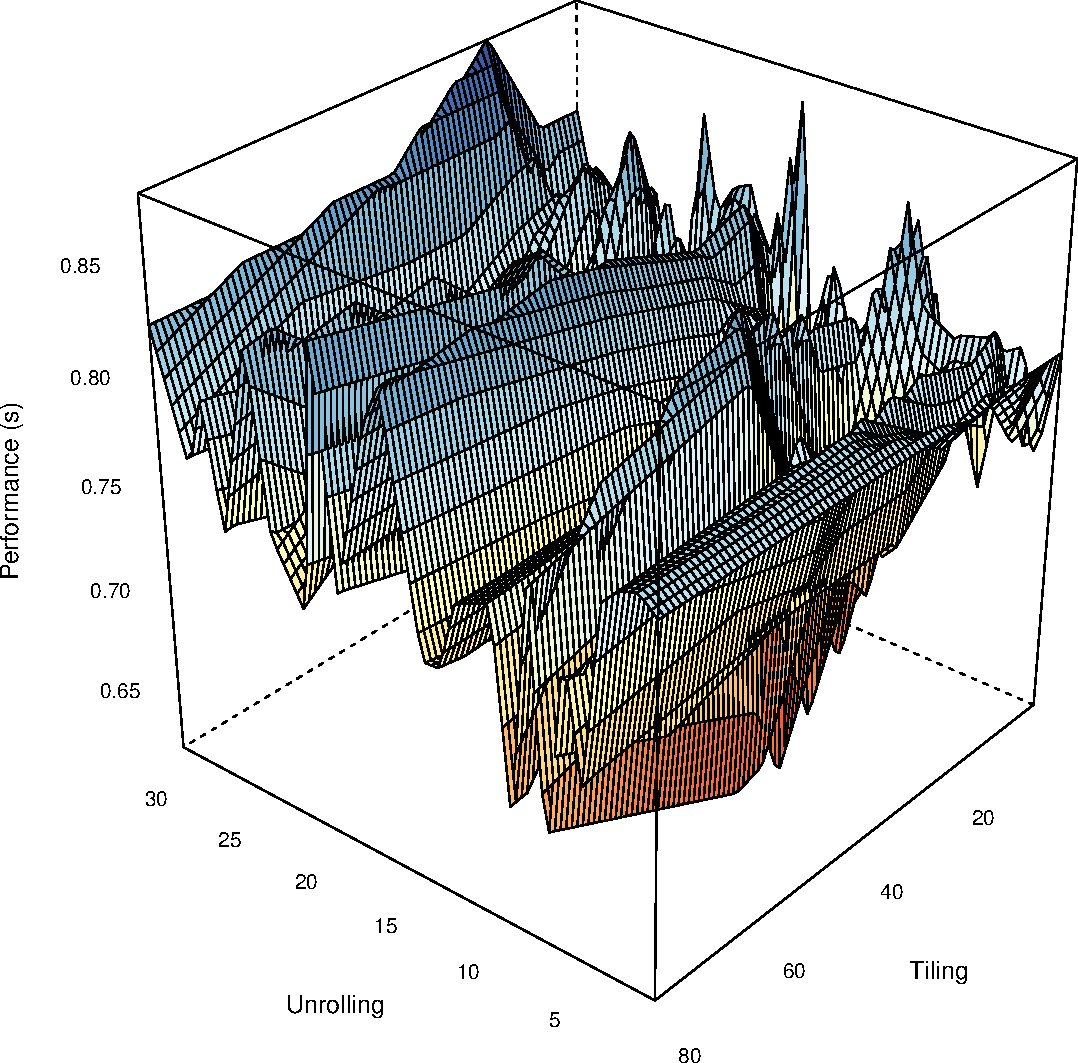
\includegraphics[width=.6\columnwidth]{../../../img/bicgkernel_averaged_search_space_edited.pdf}
\end{center}

\begin{center}
{\footnotesize
\alert{Unrolling}, \alert{tiling} and \alert{performance} for a \alert{biconjugate gradient} kernel
}
\vspace{1.3em}
\end{center}

\begin{itemize}
\item Represent the \alert{effect} of all possible
\alert{configurations} on the \alert{objectives}, can be difficult to explore,
with multiple \alert{local optima} and \alert{undefined regions}
\item \alert{Main issues} are \alert{exponential growth}, \alert{geometry}, \& \alert{measurement time}
\end{itemize}
\end{block}
\end{column}
\end{columns}

\vspace{0.2em}
\rule{\columnwidth}{0.4ex}
\vspace{-2.5em}
\begin{columns}
\begin{column}[t]{0.48\columnwidth}
\begin{block}{Design of Experiments: Exploration under a Budget}
\alert{Design of Experiments} (\alert{DoE}):
\vspace{1em}
\begin{itemize}
\item \alert{Factors} are program \alert{parameters},
and \alert{levels} are possible factor \alert{values}
\item An \alert{experiment} fixes levels,
and a \alert{design} is a \alert{selection} of experiments to \alert{run}
\item A \alert{performance model} is required to \alert{construct designs}

\vspace{1em}
\end{itemize}
\begin{columns}
\begin{column}{0.39\columnwidth}
{\scriptsize
\begin{table}[]
    \centering
    \begin{tabular}{@{\kern\tabcolsep}cccccccc@{\kern\tabcolsep}}
        \toprule
        Run & A & B & C & D & E & F & G \\ \midrule
        \cellcolor{gray!18}1 & \cellcolor{green!25}1 & \cellcolor{red!25}-1 & \cellcolor{green!25}1 & \cellcolor{red!25}-1 & \cellcolor{red!25}-1 & \cellcolor{green!25}1 & \cellcolor{green!25}1 \\
        \cellcolor{gray!18}2 & \cellcolor{green!25}1 & \cellcolor{green!25}1 & \cellcolor{green!25}1 & \cellcolor{red!25}-1 & \cellcolor{green!25}1 & \cellcolor{red!25}-1 & \cellcolor{red!25}-1 \\
        \cellcolor{gray!18}3 & \cellcolor{red!25}-1 & \cellcolor{green!25}1 & \cellcolor{red!25}-1 & \cellcolor{red!25}-1 & \cellcolor{green!25}1 & \cellcolor{green!25}1 & \cellcolor{green!25}1 \\
        \cellcolor{gray!18}4 & \cellcolor{red!25}-1 & \cellcolor{green!25}1 & \cellcolor{green!25}1 & \cellcolor{green!25}1 & \cellcolor{red!25}-1 & \cellcolor{green!25}1 & \cellcolor{red!25}-1 \\
        \cellcolor{gray!18}5 & \cellcolor{green!25}1 & \cellcolor{red!25}-1 & \cellcolor{red!25}-1 & \cellcolor{green!25}1 & \cellcolor{green!25}1 & \cellcolor{green!25}1 & \cellcolor{red!25}-1 \\
        \cellcolor{gray!18}6 & \cellcolor{green!25}1 & \cellcolor{green!25}1 & \cellcolor{red!25}-1 & \cellcolor{green!25}1 & \cellcolor{red!25}-1 & \cellcolor{red!25}-1 & \cellcolor{green!25}1 \\
        \cellcolor{gray!18}7 & \cellcolor{red!25}-1 & \cellcolor{red!25}-1 & \cellcolor{green!25}1 & \cellcolor{green!25}1 & \cellcolor{green!25}1 & \cellcolor{red!25}-1 & \cellcolor{green!25}1 \\
        \cellcolor{gray!18}8 & \cellcolor{red!25}-1 & \cellcolor{red!25}-1 & \cellcolor{red!25}-1 & \cellcolor{red!25}-1 & \cellcolor{red!25}-1 & \cellcolor{red!25}-1 & \cellcolor{red!25}-1  \\ \bottomrule
    \end{tabular}
\end{table}

}
\begin{center}
{\tiny
A \alert{Plackett-Burman} design \\[-0.5em] for \alert{7 2-level factors}
}
\end{center}
\vspace{0.2em}
\begin{itemize}
\item \alert{Results}, or \alert{responses}, can be used to
identify \alert{relevant parameters} and to \alert{fit a linear regression
model}
\end{itemize}
\end{column}
\begin{column}{0.59\columnwidth}
\begin{center}
\begin{center}
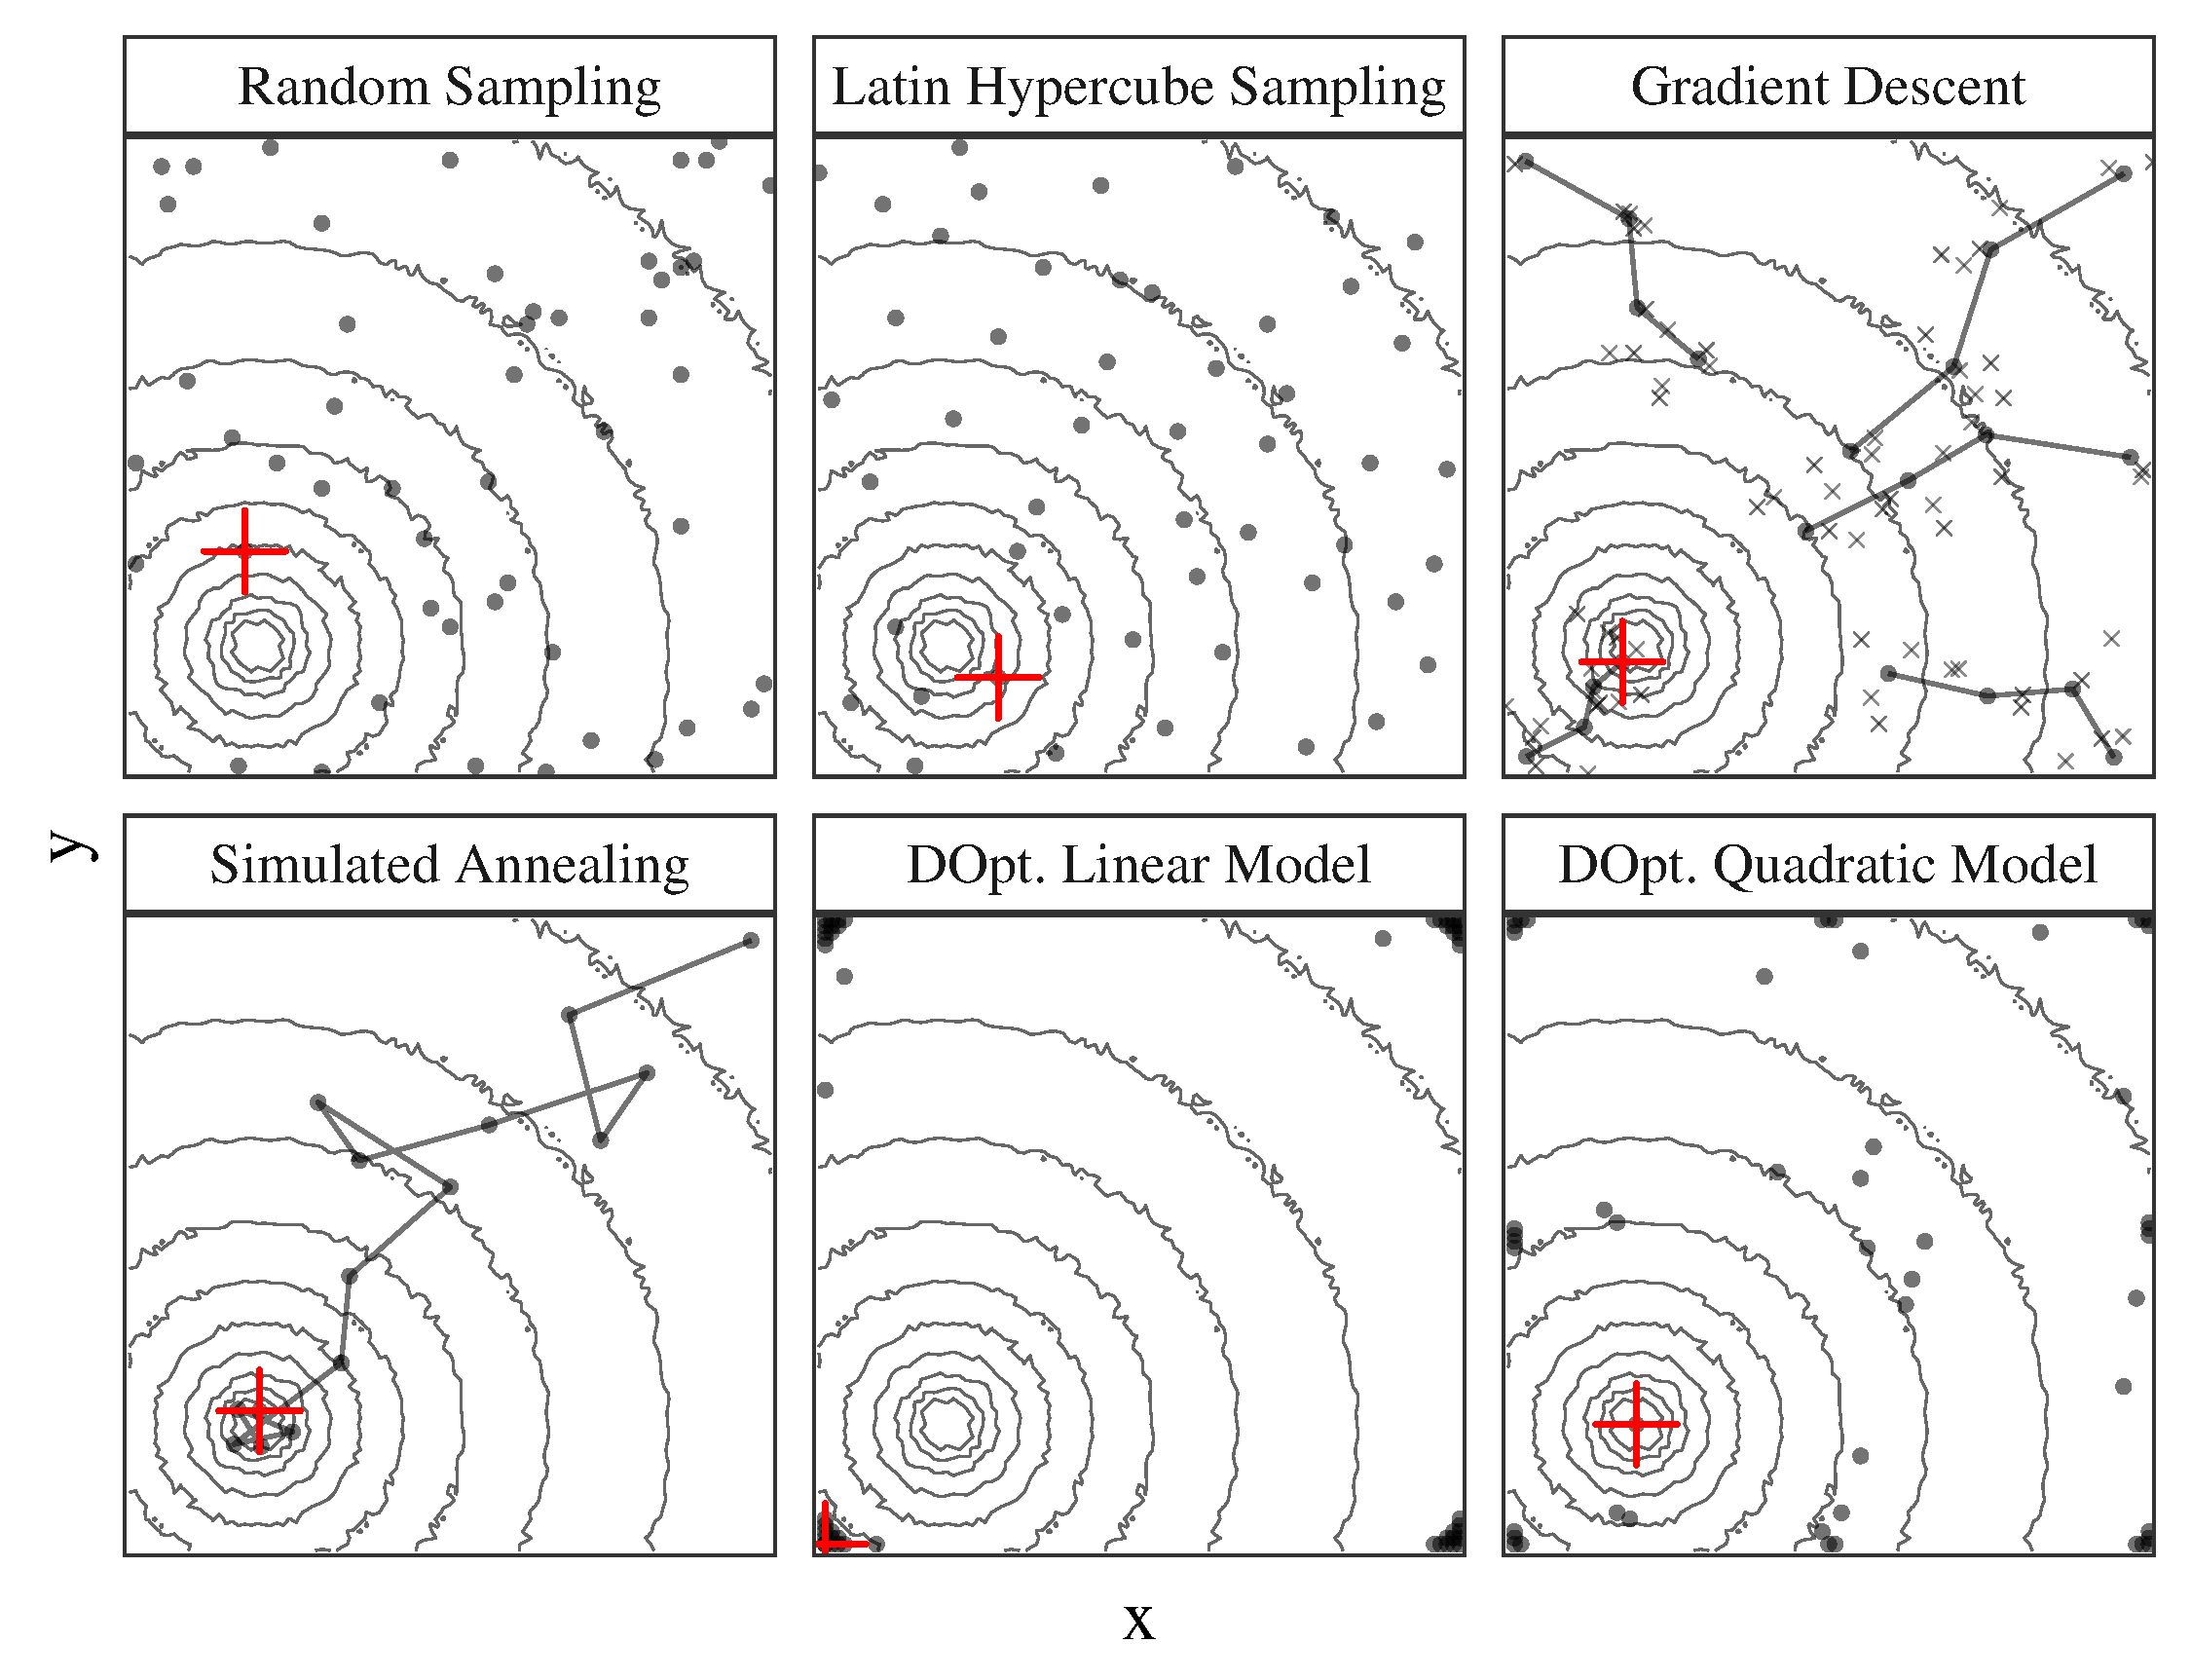
\includegraphics[width=0.98\columnwidth]{../../../img/sampling_comparison.pdf}
\end{center}
\end{center}

\begin{itemize}
\item Exploration of a search space using a \alert{fixed budget}
of \alert{50 points}, the \alert{red “+”} represents the best point found by
each strategy
\end{itemize}
\end{column}
\end{columns}
\end{block}
\end{column}
\begin{column}[t]{0.48\columnwidth}
\begin{block}{A Transparent Design of Experiments Approach}
\begin{center}
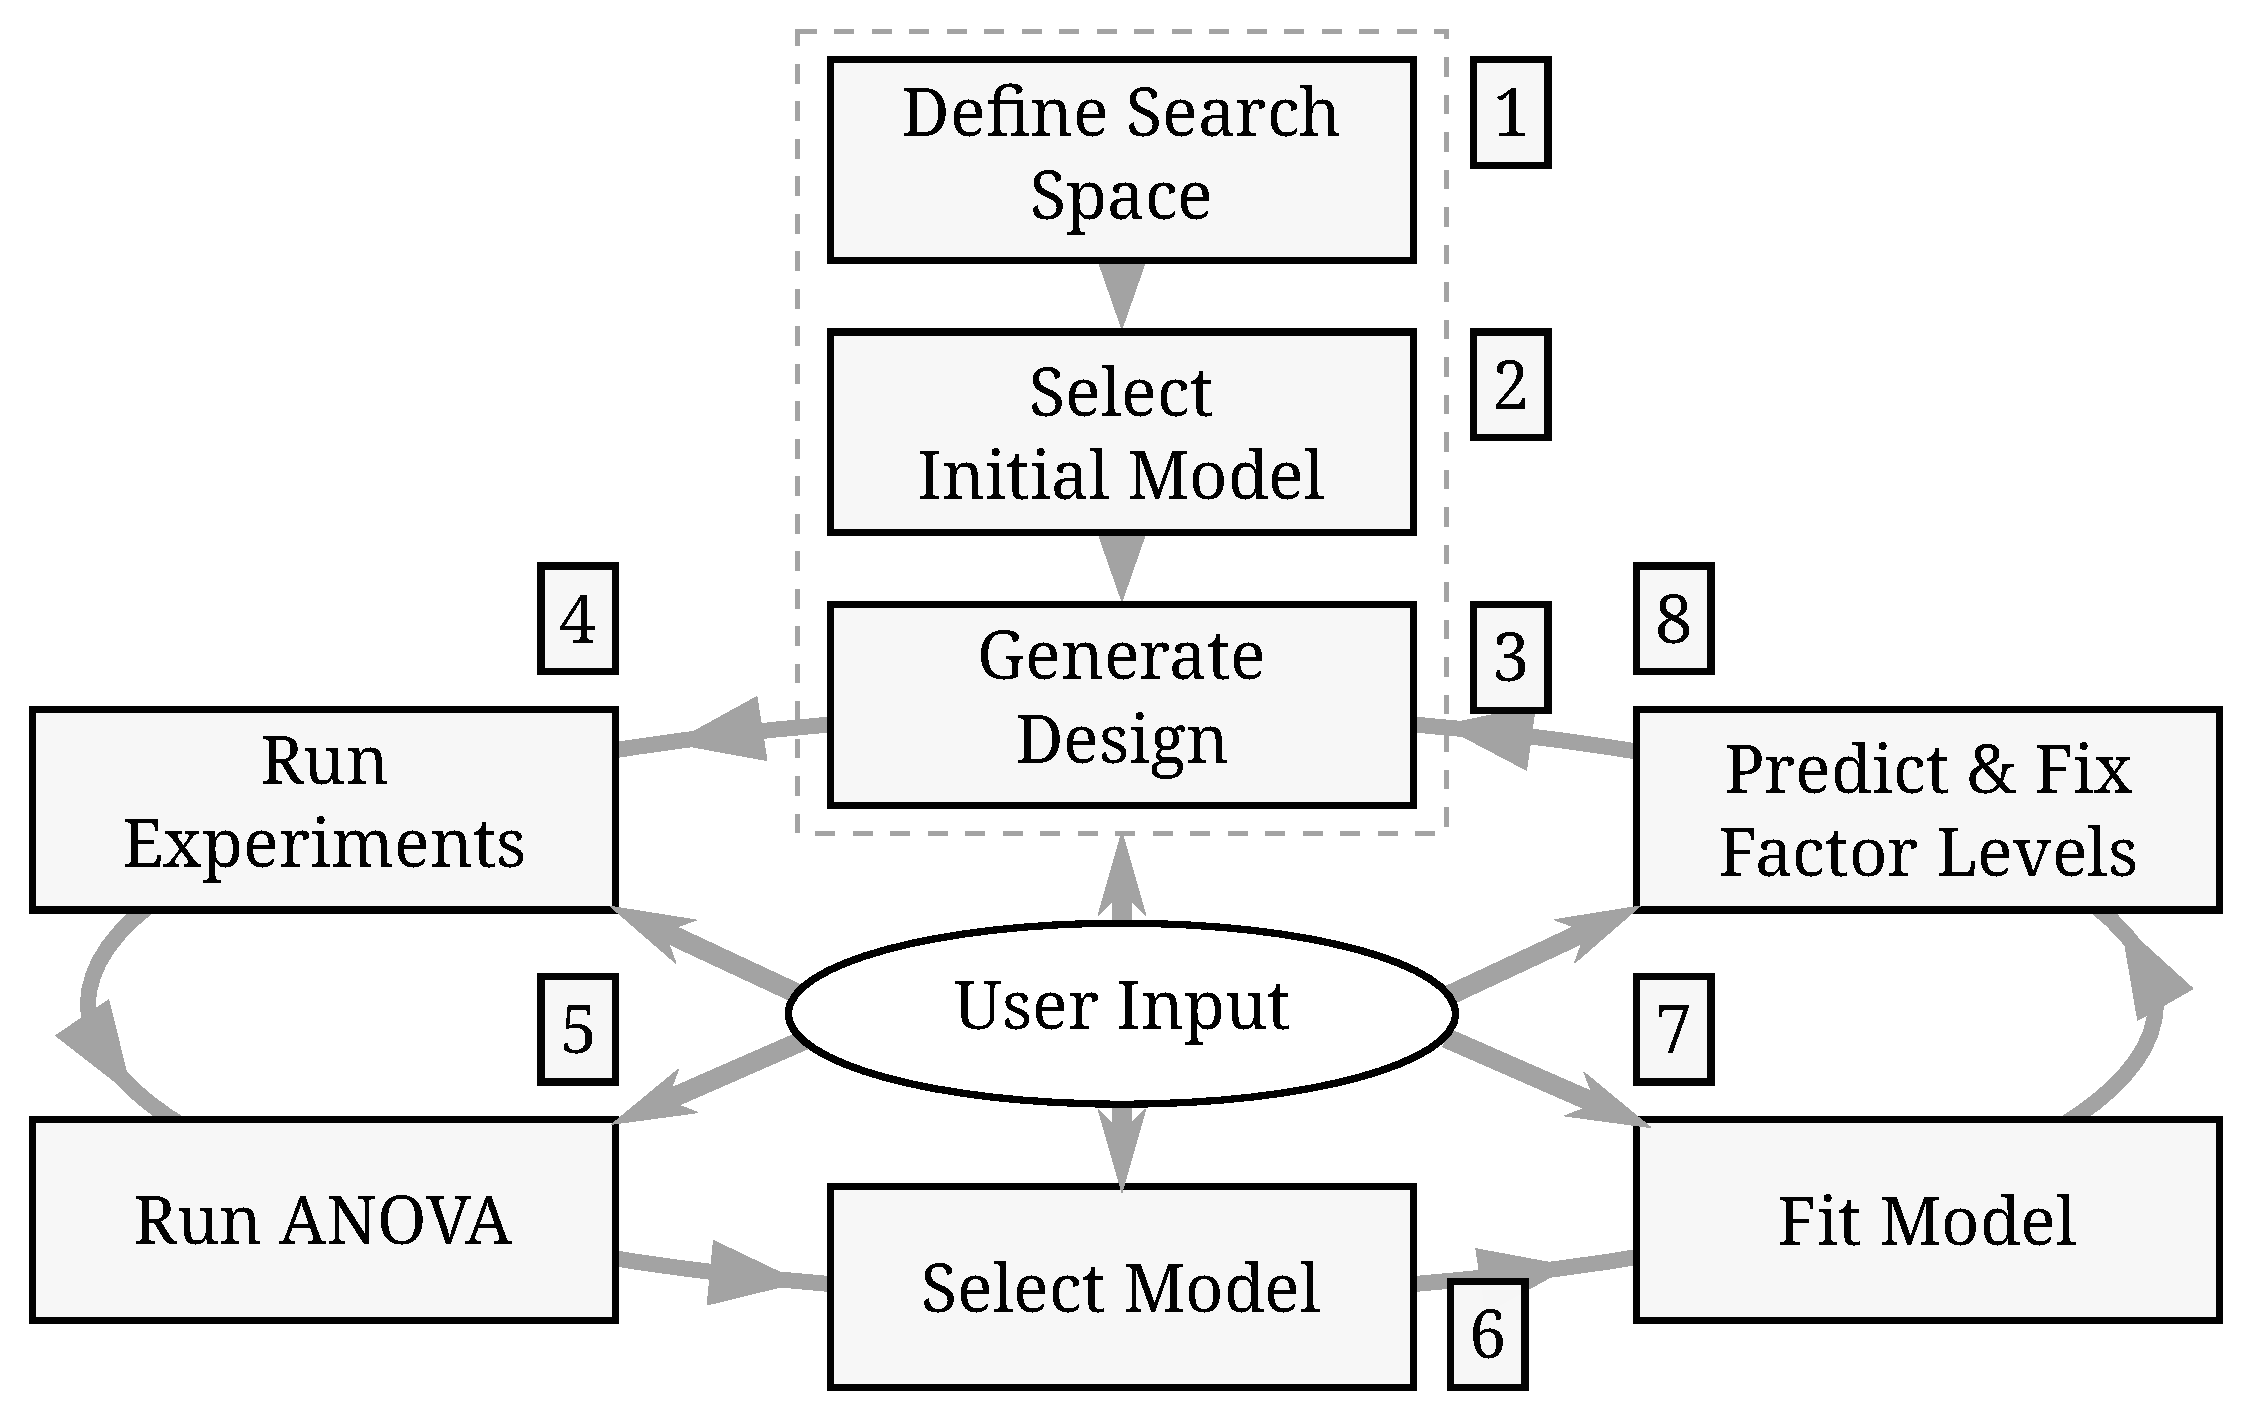
\includegraphics[width=0.8\columnwidth]{../../../img/doe_anova_strategy.pdf}
\end{center}

\vspace{1em}

\begin{itemize}
\item An \alert{initial model} is provided by the \alert{user} (steps \alert{1} \& \alert{2})
\item \alert{Design of Experiments} guides exploration (steps \alert{3} \& \alert{4})
\item \alert{Significant factors} are identified by \alert{Analysis of Variance (ANOVA)} (steps \alert{5} \& \alert{6})
\item New fitted model predicts best value for significant factors (steps \alert{7} \& \alert{8})

\begin{center}
  {\normalsize
    \colorbox{WinterSkin}{\alert{\vphantom{g}Transparent}: {\small \alert{factor} and \alert{level} selections based on \alert{ANOVA}}} \\[0.2em]
    \colorbox{WinterSkin}{\alert{Parsimonious}: {\small DoE \alert{decreases measurements}}}
  }
\end{center}
\end{itemize}
\end{block}
\end{column}
\end{columns}
\vspace{0.2em}
\rule{\columnwidth}{0.4ex}
\vspace{-2.5em}
\begin{columns}
\begin{column}[t]{0.48\columnwidth}
\begin{block}{A Motivating Result on a GPU Kernel}
\begin{columns}
\begin{column}{0.49\columnwidth}
\begin{itemize}
\item Kernel \alert{factors}:
\vspace{0.6em}
\begin{table}[htbp]
\centering
\tiny
\begin{tabular}{llp{0.3\columnwidth}}
\toprule
Factor & Levels & Short Description\\
\midrule
\texttt{vector\_length} & \(2^0,\dots,2^4\) & Size of support arrays\\
\texttt{load\_overlap} & \textit{true}, \textit{false} & Load overlaps in vectorization\\
\texttt{temporary\_size} & \(2,4\) & Byte size of temporary data\\
\texttt{elements\_number} & \(1,\dots,24\) & Size of equal data splits\\
\texttt{y\_component\_number} & \(1,\dots,6\) & Loop tile size\\
\texttt{threads\_number} & \(2^5,\dots,2^{10}\) & Size of thread groups\\
\texttt{lws\_y} & \(2^0,\dots,2^{10}\) & Block size in \(y\) dimension\\
\bottomrule
\end{tabular}
\end{table}
\end{itemize}
\end{column}

\begin{column}{0.49\columnwidth}
\begin{itemize}
\item Initial \alert{performance model}:
{\tiny
  \begin{align}
    time\_per\_pixel \sim & \; y\_component\_number + \frac{1}{y\_component\_number} \; + \nonumber \\
    & \; load\_overlap + temporary\_size \; + \nonumber \\
    & \; vector\_length + lws\_y + \frac{1}{lws\_y} \; + \nonumber \\
    & \; elements\_number + threads\_number  \; + \nonumber \\
    & \; \frac{1}{elements\_number} + \frac{1}{threads\_number}\text{.} \nonumber
  \end{align}
}

\begin{itemize}
\item This \alert{simple case} had known \alert{valid search space} and
\alert{global optimum}, and \alert{fixed budget}
\end{itemize}
\end{itemize}
\end{column}
\end{columns}
\vspace{1em}
\begin{center}
{\small
Our approach (\alert{DLMT}) was always \alert{within 1\% of the optimum}
}
\end{center}
\begin{center}
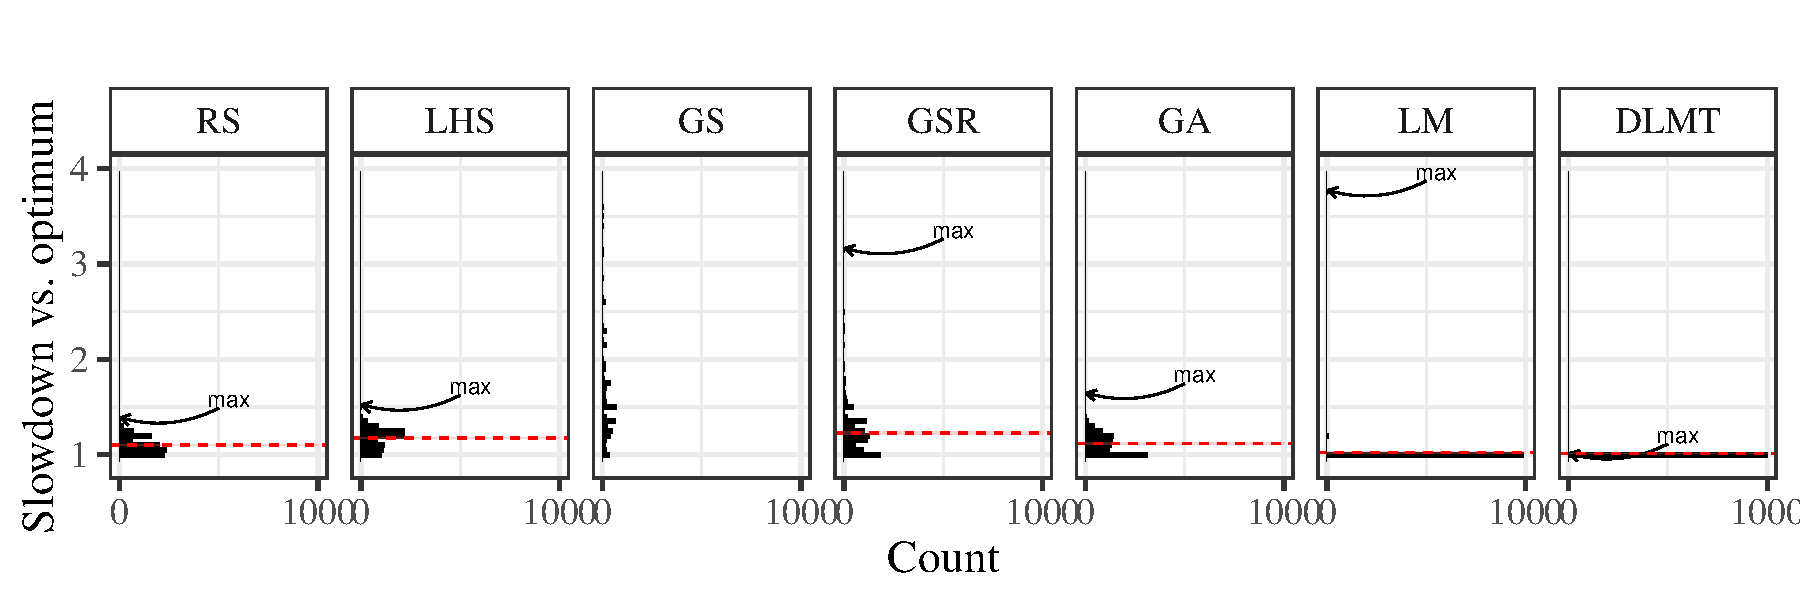
\includegraphics[width=0.9\columnwidth]{../../../img/comparison_histogram.pdf}
\end{center}

\begin{table}[htbp]
\centering
\tiny
\begin{tabular}{p{0.09\columnwidth}p{0.09\columnwidth}p{0.09\columnwidth}p{0.09\columnwidth}p{0.09\columnwidth}p{0.09\columnwidth}p{0.09\columnwidth}}
\toprule
RS & LHS & GS & GSR & GA & LM & DLMT\\
\midrule
Random Sampling & Latin Hyper Square & Greedy Search & Greedy with Restart & Generic Algorithm & Linear Model & Our DoE Approach\\
\bottomrule
\end{tabular}
\end{table}
\end{block}
\end{column}
\begin{column}[t]{0.48\columnwidth}
\begin{block}{ \vphantom{g}Extensive Evaluation on the SPAPT Benchmark}
\begin{itemize}
\item \alert{SPAPT} is an \alert{autotuning benchmark} for \alert{CPU kernels}, with \alert{search space sizes}
between \alert{\(10^7\) and \(10^{36}\)}
\item We evaluated \alert{DLMT} on \alert{17 kernels} (\alert{3} shown below)
using \alert{the same initial performance model}, and \alert{fixed budget}

\vspace{0.3em}
\begin{center}
{\small
Our approach (\alert{DLMT}) achieved \alert{good speedups} using
  \\[0.3em] a \alert{smaller budget}, while \alert{exploring better
configurations}
}
\end{center}
\begin{center}
\begin{center}
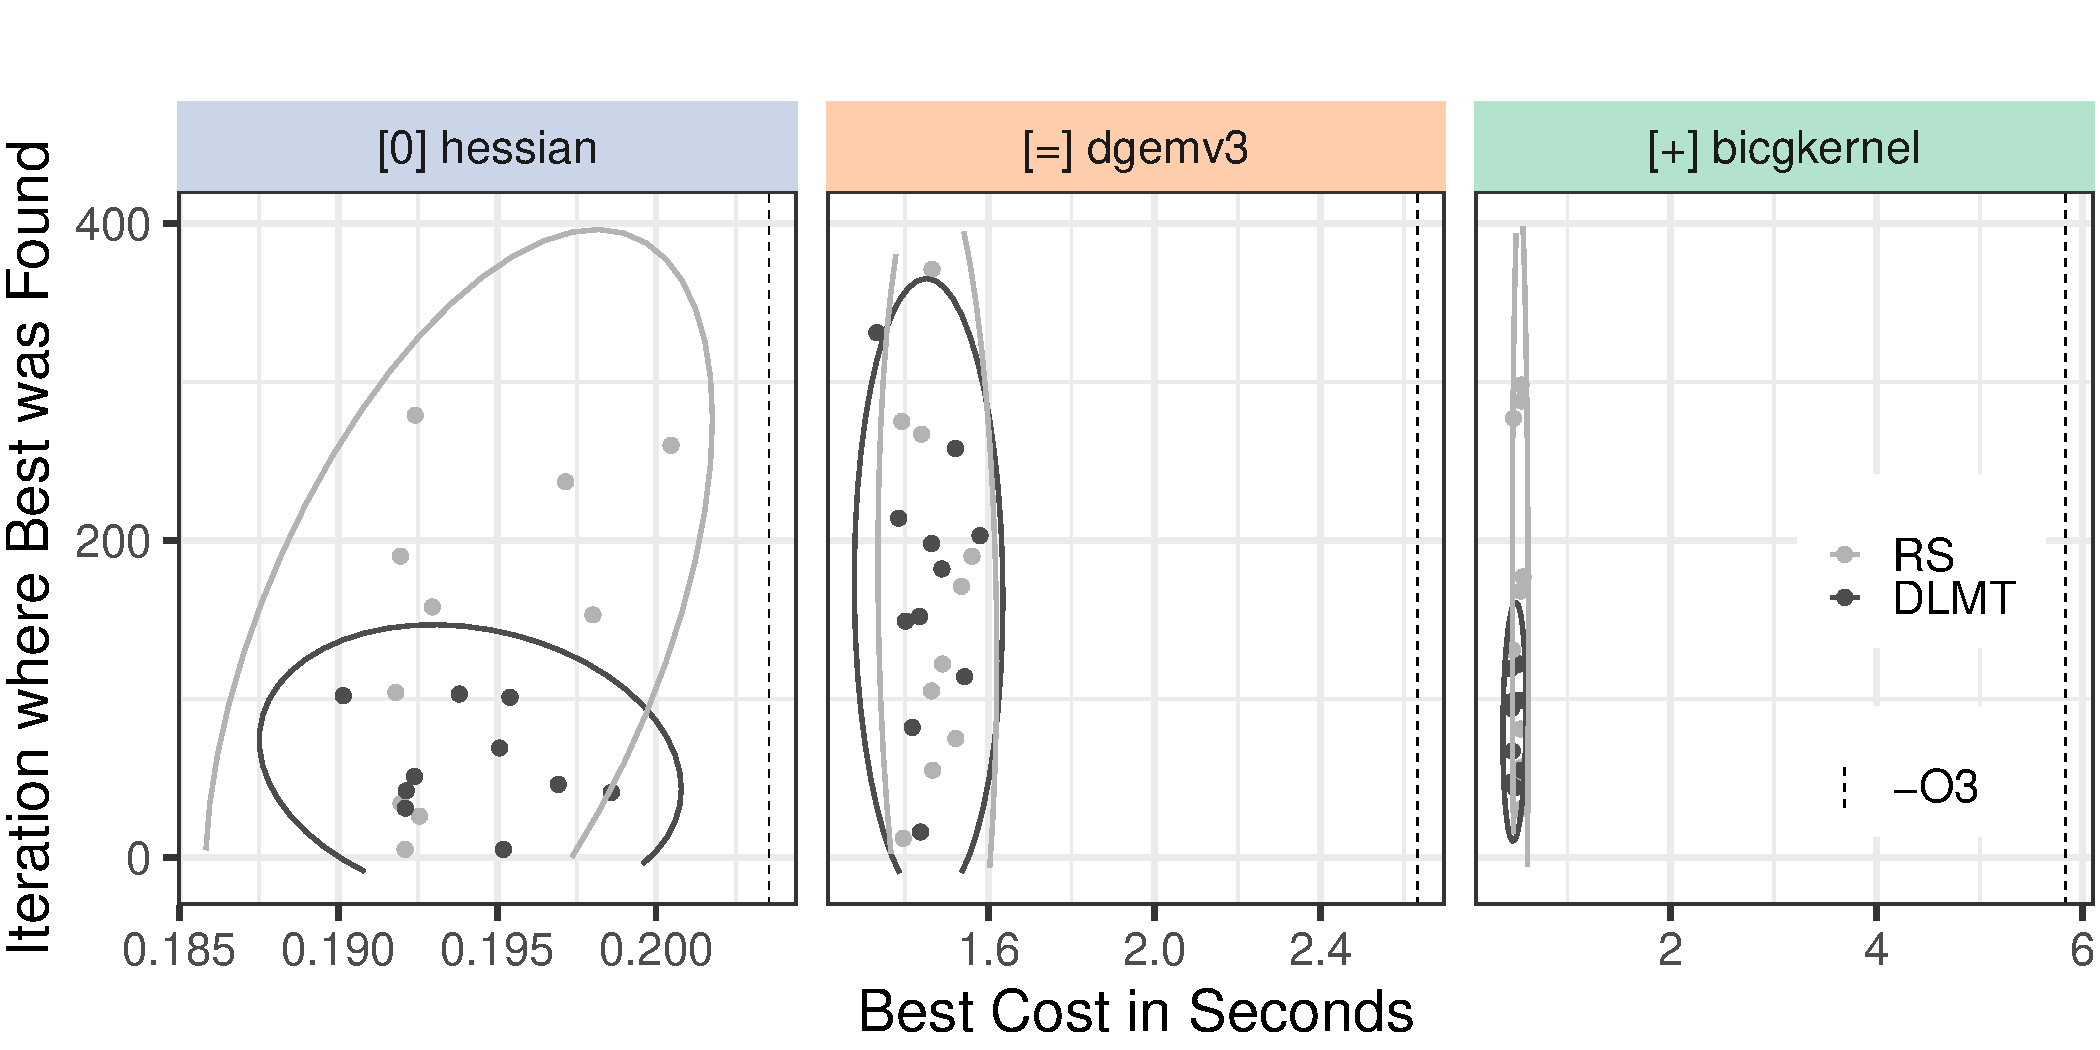
\includegraphics[width=0.85\columnwidth]{../../../img/iteration_best_comparison.pdf}
\end{center}
\end{center}

\begin{center}
\begin{center}
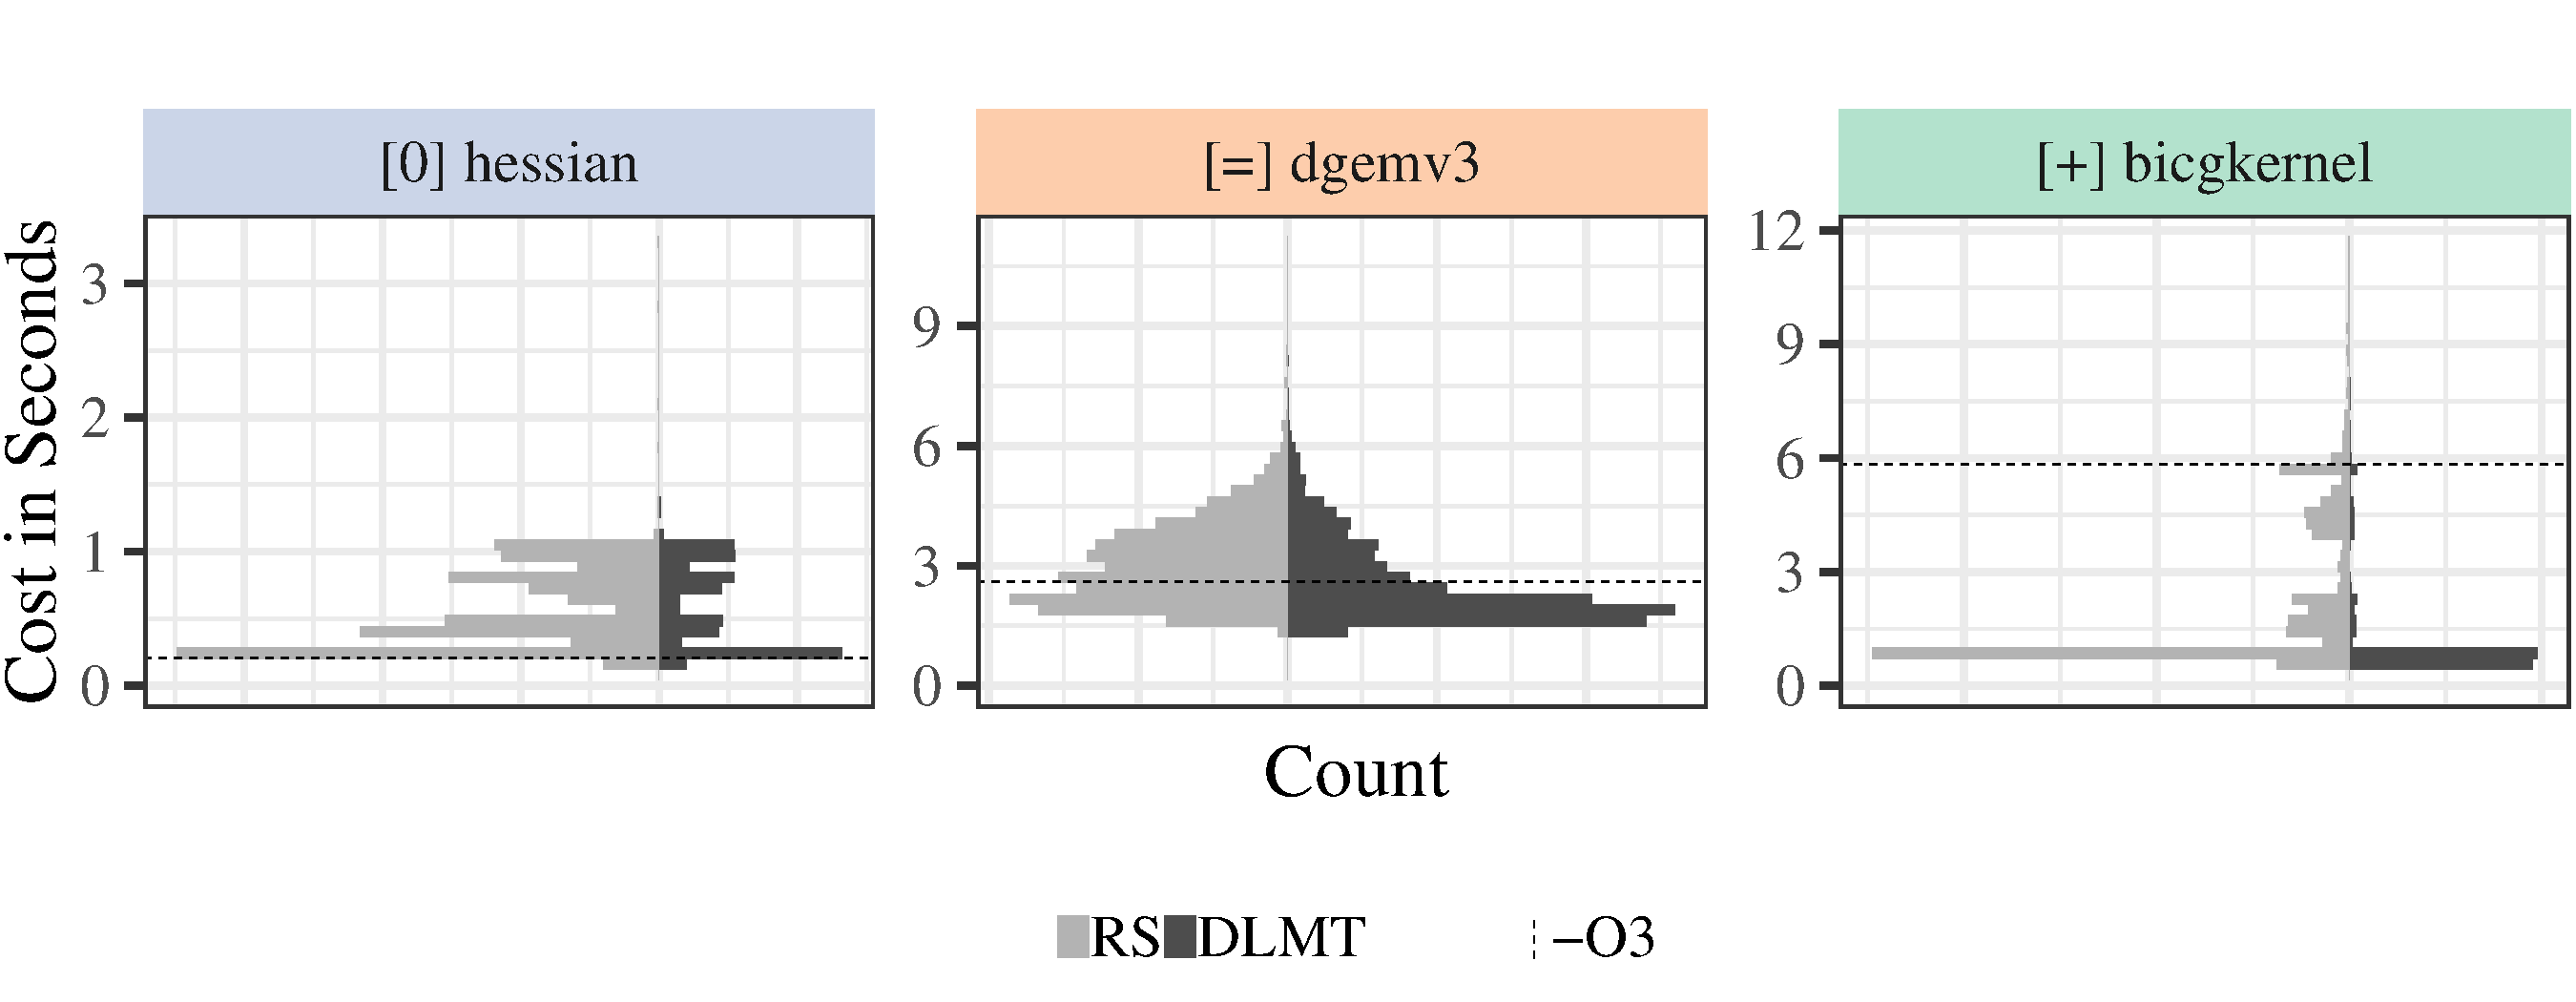
\includegraphics[width=0.85\columnwidth]{../../../img/split_histograms.pdf}
\end{center}
\end{center}
\end{itemize}
\end{block}
\end{column}
\end{columns}
\begin{columns}
\begin{column}{0.9\columnwidth}
\begin{flushleft}
\vspace{1.3em}
  {\small
    \textit{$^{1}$University of São Paulo, São Paulo, Brazil, with CAPES Funding \\
      $^{2}$University of Grenoble Alpes, Inria, CNRS, Grenoble INP, LJK 38000 Grenoble, France \\[-0.2em]
      $^{3}$University of Grenoble Alpes, CNRS, Inria, Grenoble INP, LIG 38000 Grenoble, France
    }
  }
\end{flushleft}
\end{column}
\begin{column}{0.1\columnwidth}
\end{column}
\end{columns}
\end{column}

\begin{column}{0.09\columnwidth}
\end{column}
\end{columns}
\end{frame}
\end{document}
